\documentclass{beamer}

\mode<presentation>
 {\usetheme{CambridgeUS}
  \usecolortheme{beaver}
  \setbeamercovered{transparent}
  % appearance of bullets
  \useinnertheme{rectangles}
  \definecolor{mybullets}{rgb}{0.6,0.0,0.0}
  \setbeamercolor{structure}{fg=mybullets}

  \definecolor{mycolor}{rgb}{0.2,0.2,0.2}
  % bars
  %\setbeamercolor{section in toc}{fg=black,bg=white}
  %\setbeamercolor{alerted text}{fg=mycolor!80!gray}
  %\setbeamercolor*{palette primary}{fg=mycolor!60!black,bg=gray!30!white}
  %\setbeamercolor*{palette secondary}{fg=mycolor!70!black,bg=gray!15!white}
  %\setbeamercolor*{palette tertiary}{bg=mycolor!80!black,fg=gray!10!white}
  %\setbeamercolor*{palette quaternary}{fg=mycolor,bg=gray!5!white}
  %\setbeamercolor*{sidebar}{fg=mycolor,bg=gray!15!white}

  \setbeamercolor*{palette sidebar primary}{fg=mycolor!10!black}
  \setbeamercolor*{palette sidebar secondary}{fg=white}
  \setbeamercolor*{palette sidebar tertiary}{fg=mycolor!50!black}
  \setbeamercolor*{palette sidebar quaternary}{fg=gray!10!white}

  \setbeamercolor{titlelike}{parent=palette primary,fg=mycolor}
  \setbeamercolor{frametitle}{bg=gray!10!white}
  \setbeamercolor{frametitle right}{bg=gray!60!white}

  \setbeamercolor*{separation line}{}
  \setbeamercolor*{fine separation line}{}
}

 \def\Tiny{\fontsize{5pt}{5pt}\selectfont}
 \renewcommand{\arraystretch}{1.2}

% just show sections and subsections in table of contents
\setcounter{tocdepth}{2}


\usepackage[english]{babel}
\usepackage[latin1]{inputenc}

\usepackage{times}
\usepackage[T1]{fontenc}
\usepackage{eurosym}

% TODO: Milestone 1 huebsch unterbringen
\title[NES Project: Milestone Presentation]{Position Sensing and Imitation\\Milestone Presentation}

\author[Koslowski, Schmieder, Birk]{Konstantin Koslowski, Mathis Schmieder, Moksha Birk}

\institute[]
{TU Berlin \\
 Department of Telecommunication Systems \\
 Telecommunication Networks Group \\
}

\date{May 22nd, 2015}

\pgfdeclareimage[height=0.5cm]{university-logo}{tu-tkn-logo.jpg}
\logo{\pgfuseimage{university-logo}}

\begin{document}

\begin{frame}
  \titlepage
\end{frame}

\section{Networked Embedded Systems}
\subsection{Project}

\begin{frame}
  \frametitle{Goal Statement}
	\begin{itemize}
		\item \textbf{Goal:} Mimic position and motion of a plate
		\vfill
		\item \textbf{Sensing:} 3D MEMS attitude sensor embedded in a plate
		\item \textbf{Communicating:} Implement industrial bus, likely ModBus
		\item \textbf{Actuating:} Rotate a plate using motors
	\end{itemize}
\end{frame}

\subsection{Functional Specification}
\begin{frame}
  \frametitle{Overview}
\begin{figure}
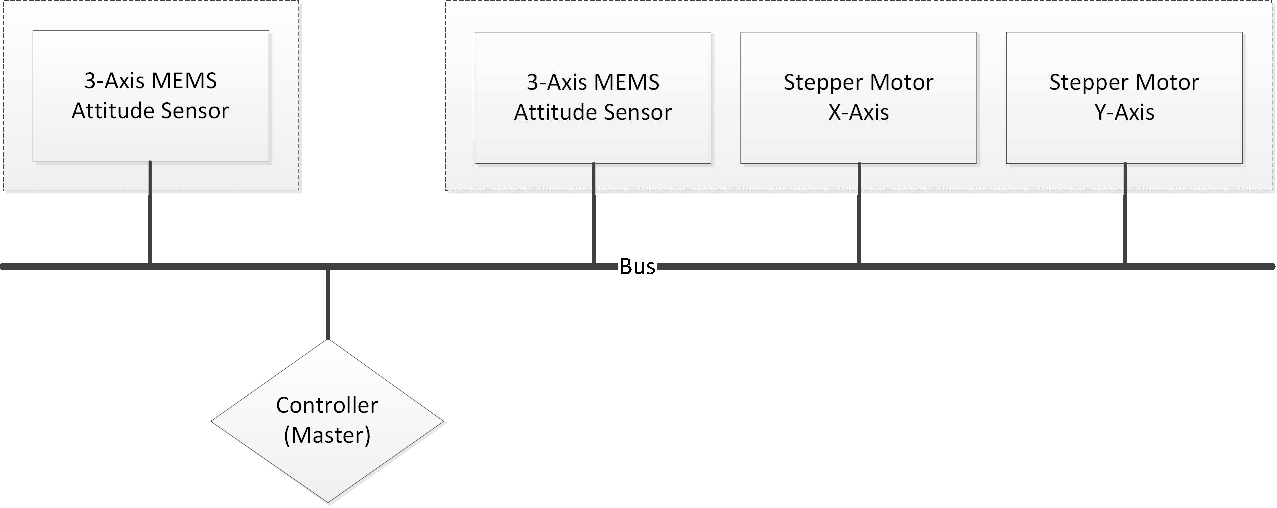
\includegraphics[width=\textwidth]{functionalspecification.pdf} 
\caption{Diagram of the Functional Specification}
\end{figure}
\end{frame}

\begin{frame}
	\frametitle{Sensing}
	\begin{itemize}
		\item \textbf{Sensor:} LSM303DLH 3D Compass and Accelerometer
		\item \textbf{Controller:} Arduino Pro Micro
		\item \textbf{Communication:} TTL to RS-485 Module
		\item Attitude in 3 dimensions is sensed and communicated via bus
	\end{itemize}
\end{frame}

\begin{frame}
	\frametitle{Computation \& Communication}
	\begin{itemize}
		\item \textbf{Controller:} Beagle Bone Black
		\item \textbf{Communication:} TTL to RS-485 Module
		\item \textbf{Bus Protocol:} Industrial bus with open implementation, likely ModBus
		\item Controller receives sensor data \& computes desired motor movement
	\end{itemize}
\end{frame}

\begin{frame}
	\frametitle{Actuation}
	\begin{itemize}
		\item \textbf{Motor:} NEMA 11 Stepper
		\item \textbf{Controller:} Arduino Pro Micro, Pololu A4988 Motor Driver
		\item \textbf{Communication:} TTL to RS-485 Module
		\item Motor is rotated the desired amount
	\end{itemize}
\end{frame}

\begin{frame}
  \frametitle{Hardware Components}
	\begin{itemize}
		\item 2x LSM303DLH MEMS Sensors, 10 Euro each
		\item 3x Arduino Pro Micro,  5 Euro each
		\item 2x A4988 Motor Driver, 3 Euro each
		\item 2x NEMA11 Stepper Motors, 25 Euro each
		\item 4x TTL to RS-485 Modules, <1 Euro each
		\item Beagle Bone Black
	\end{itemize}
\end{frame}

\subsection{Milestones}
\begin{frame}
  \frametitle{Major Milestones}
	\begin{itemize}
		\item \textbf{Sensing:} Read and process MEMS data on Arduino\\
			\small{Konstantin Koslowski}
		\item \textbf{Actuation:} Control stepper motors\\
			\small{Mathis Schmieder, Konstantin Koslowski}
		\item \textbf{Mechanics:} Construct movable plate\\
			\small{Mathis Schmieder}
		\item \textbf{Communication:} Implement industrial bus\\
			\small{Moksha Birk}
		\item \textbf{Controller:} Bus master, main computational unit\\
			\small{Moksha Birk}
	\end{itemize}
\end{frame}

\subsection{Discussion}
\begin{frame}
	\frametitle{Thanks for your attention!}
	\huge{Questions? Ideas? Suggestions?}
\end{frame}

\end{document}
